
\ifintegriereaufgaben

\section*{Diskrete Fouriertransformation}\label{MA2-diskrete-fouriertransformation-aufgaben}
Regeln und Beispiele, die zur Bearbeitung der Aufgaben hilfreich sind, finden Sie im Skript\wennreferenzvorhanden{MA2-diskrete-fouriertransformation}{ (Abschnitt \abschnittsverweis{MA2-diskrete-fouriertransformation})} und, falls Sie nicht weiterkommen, schauen Sie \hyperref[MA2-diskrete-fouriertransformation-loesungen]{hier}.
\else
\section{Diskrete Fouriertransformation}\label{MA2-diskrete-fouriertransformation-aufgaben}

Regeln und Beispiele zu diesen Aufgaben finden Sie im Skript. Die L�sungen finden Sie \hyperref[MA2-diskrete-fouriertransformation-loesungen]{hier}.
\fi

\begin{exabox}[Orthogonalit�t]
	Bei der Digitalsignal�bertragung werden energiebegrenzte Signale betrachtet. Das Skalarprodukt zweier Signale bzw. die Norm eines Signals sind hierbei wie folgt definiert:
	\begin{eqnarray*}
		\langle s_i, s_k\rangle &=& \int\limits_{-\infty}^{\infty} s_i(t) \cdot s_k(t) \, \mathrm{d}t\,,\\[1ex]
		\|s\| &=& \sqrt{\langle s,s \rangle}\,.
	\end{eqnarray*}
	Betrachten Sie die folgenden drei energiebegrenzten Signale:
	\begin{center}
	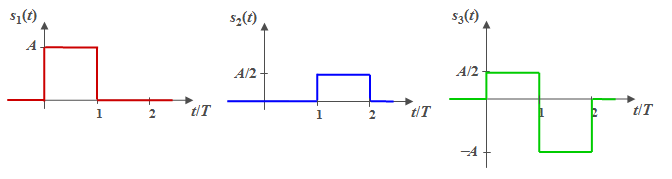
\includegraphics[width=0.7\textwidth]{../Mathematik_2/Bilder/dft_rechtecksignale_linearkombination.png}
\end{center}
	\begin{itemize}
		\item[(a)] Wie lauten die Abbildungsvorschriften der Signale $s_1, s_2$ und $s_3$?
		\item[(b)] Berechnen Sie die Normen der Signale $s_1$ und $s_2$.
		\item[(c)] Konstruieren Sie aus den Signalen $s_1$ und $s_2$ ein Orthonormalsystem.
		\item[(d)] Zerlegen Sie das Signal $s_3$ bez�glich des Orthonormalsystems und bestimmen Sie die vektoriellen Repr�sentanten der Ausgangssignale bez�glich des Orthonormalsystems.
	\end{itemize}
\end{exabox}

\begin{exabox}[�quivalenz reelle und komplexe Fourierreihe]
	Zeigen Sie, dass es zur komplexen Fourierreihe eine �quivalente reelle Darstellung gibt und geben Sie an, wie sich die Koeffizienten ineinander �berf�hren lassen. Hinweis: Benutzen Sie die Eulersche Identit�t.%  \( e^{i\,k\omega t} =  \cos(k \omega_0 t) + i \sin(k \omega_0 t) \,. \)
\end{exabox}

\begin{exabox}[Matlab Funktion: Fourierreihe Rechtecksignal]
%	16.6 p.427
	Die Stromst�rke in einem elektrischen Stromkreis verh�lt sich in vielen F�llen wie ein Rechtecksignal. Ein Rechtecksignals ist die periodische Fortsetzung der folgenden Funktion \(f: [0,T) \to f(t)\,,\) wobei

	\[ f(t) = \begin{cases} &A_0, \quad 0\leq t \leq T/2\,,\\ -&A_0, \quad T/2\leq t < T\,. \end{cases} \]

\begin{minipage}{0.5\textwidth}
	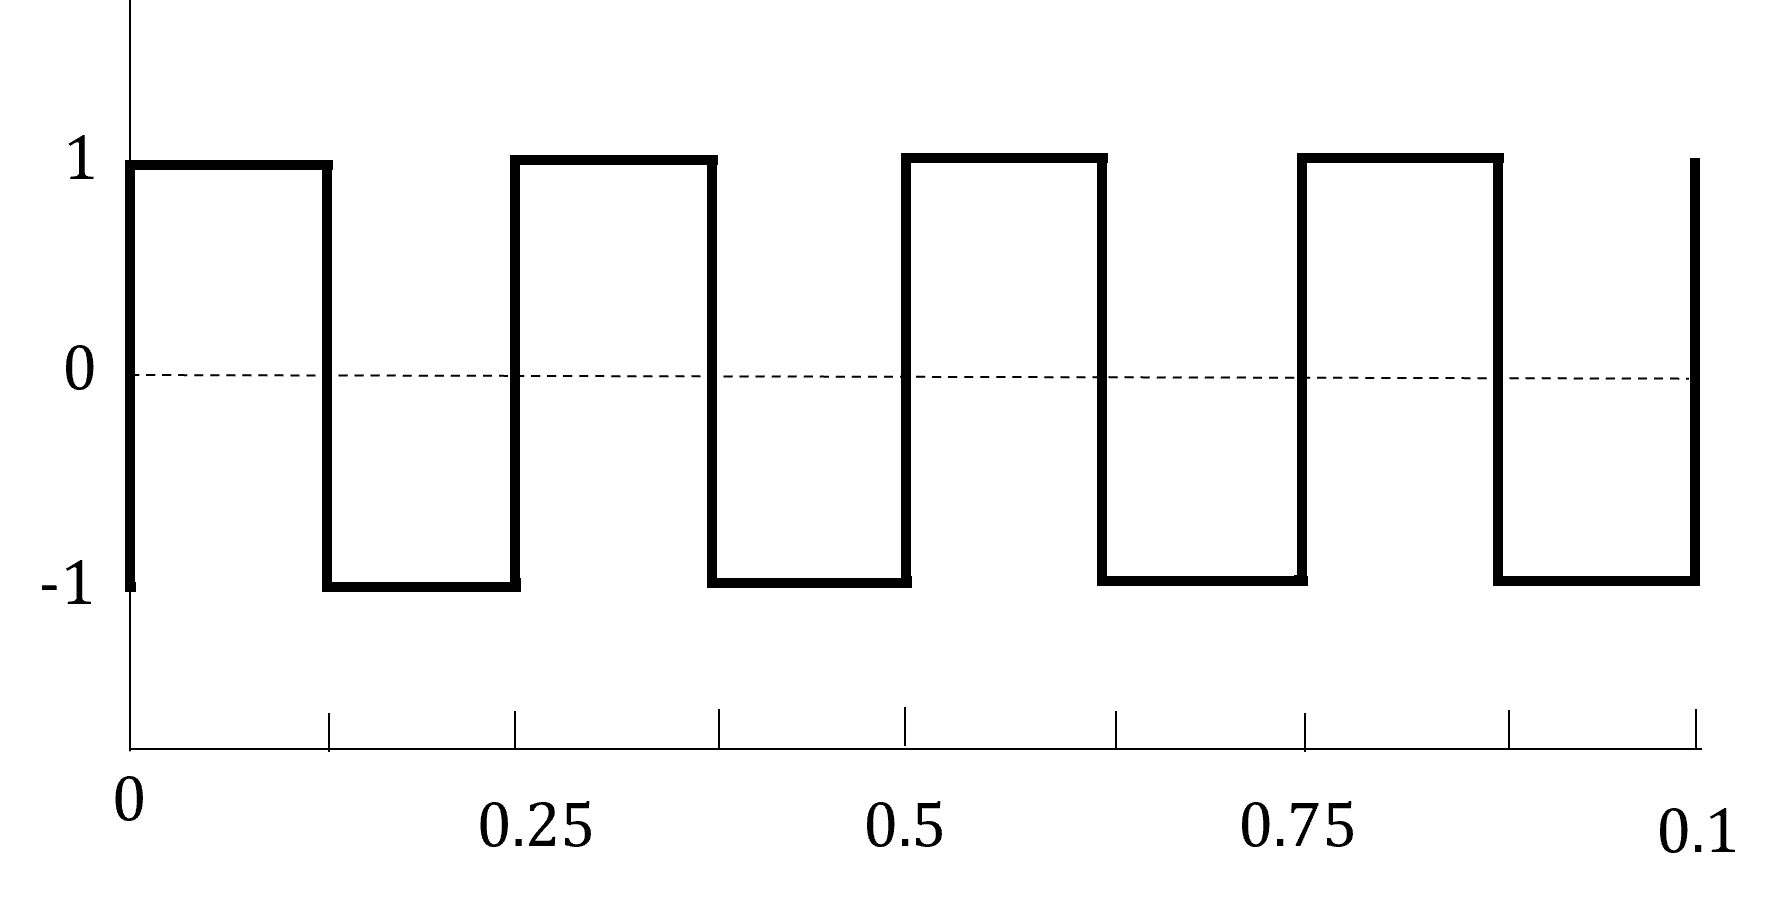
\includegraphics[width=\textwidth]{../Mathematik_2/Bilder/dft_rechtecksignal_wechselndes_vorzeichen.png}
\end{minipage}
\begin{minipage}{0.5\textwidth}
	Das Bild zeigt den Graph von \(f\) f�r \(A_0=1\,, \, T=1/4\):
	\[ f(t) = \begin{cases} &1, \quad 0\leq t \leq 1/8\,,\\ -&1, \quad 1/8\leq t < 1/4\,. \end{cases} \]
\end{minipage}

\begin{itemize}
	\item[(a)] Analysieren Sie die Symmetrie des Signals \(f\) und berechnen Sie anschlie�end die reelle Fourierreihe von \(f\).
	\item[(b)] Schreiben Sie die Matlab Funktion
		\begin{lstlisting}
		function [t,FR] = FourierSquare(A0, T, n)
		\end{lstlisting}
		\(\verb-FourierSquare-\) erh�lt als Eingabedaten die Amplidude \(A_0\), die Periode \(T\) des Rechtecksignals und den Grad \(n\) des gew�nschten Fourierpolynoms. \(\verb-FourierSquare-\) erzeugt ein Bild, auf dem
		\begin{itemize}
			\item die Graphen der ersten \(n\) Terme der Fourierreihe �ber dem Intervall \([0,T)\) abgebildet sind, jede Funktion wird mit d�nner, gestrichelter roter Linie gemalt, und,
			\item der Graph des Fourierpolynoms vom Grad \(n\) mit dicker, schwarzer Linie gemalt (\verb+'k-','linewidth',2+).
		\end{itemize}
\end{itemize}
\end{exabox}

\begin{exabox}[Minimierungsproblem]
	Es sei \(f\) ein \(2\pi\)-periodisches Signal. Zeigen Sie, dass das Fourierpolynom
	\[
	g_n(t) = \dfrac{a_0}{2} + \sum\limits_{k=1}^n a_k \cos(k\cdot t) + b_k \sin(k\cdot t), \quad a_k = \dfrac{1}{\pi} \int\limits_{-\pi}^{\pi} f(t)\cdot \cos(k\cdot t)\,\mathrm{d} t, \; b_k = \dfrac{1}{\pi} \int\limits_{-\pi}^{\pi} f(t)\cdot \cos(k\cdot t)\,\mathrm{d} t\,,\]
	unter allen trigonometrischen Polynomen vom Grad \(n\) den kleinsten Abstand zu \(f\) hat. Das Abstandsma� ist \[ ||f-g||_2 = \sqrt{ \int\limits_{-\pi}^\pi |f(t) - g(t)|^2 \, \mathrm{d} t }\,.\]
\end{exabox}

\begin{exabox}[Interpolationseigenschaft]
	Gegeben sind \(N\) Samples \(\left( t_n, f_n\right), \; n=0,\cdots,N-1,\) eines \(T\)-periodischen Signals \(f\). Zeigen Sie, dass die DFT ein Fourierpolynom definiert, das alle Samples interpoliert.
\end{exabox}

\begin{exabox}[DFT per Hand]
	Nehmen wir an das kontinuierlich gegebene Signal
	\[ f: t\mapsto 5 + 2\cos(2\pi t - \pi/2) + 3\cos(4\pi t) \]
	wird pro Sekunde vier Mal abgetastet.
	\begin{itemize}
		\item[(a)] Bestimmen Sie die Samples, die in einer Sekunde gemessen werden.
		\item[(b)] Bestimmen Sie die diskrete Fourier-Transformation und zeigen Sie, dass sich die diskrete Founier-Transformation als Matrix-Vektor-Multiplikation schreiben l��t.
		\item[(c)] Wie l��t sich das Ergebnis interpretieren?
	\end{itemize}
\end{exabox}

\begin{exabox}[Matlab: Diskrete Fouriertransformation (DT)] % p.428 16.11 standard
	Gegeben ist das Signal \[ f: t\mapsto  \cos\left(2\pi \cdot \dfrac{25}{2} \cdot t\right) + \cos\left( 2\pi \cdot 25 \cdot t\right)\,. \] Generieren Sie \(64\) Samples mit Schrittweite \(\Delta t = 0.01\, \mathrm{s}\).
	\begin{itemize}
		\item[(a)] Bestimmen Sie die Abtastrate \(f_s\), die Zeitspanne der Aufzeichnung \(t_n\), die Nyquist Freqzenz \(f_{\max}\) und die minimale detektierbare Frequenz \(f_{\min}\).
		\item[(b)] Bestimmen Sie mit Hilfe der Matlab Funktion \(\verb-fft-\) die diskrete Fouriertransformation ausgehend von den \(64\) Samples und plotten Sie das Spektrum.
	\end{itemize}
\end{exabox}

\begin{exabox}{Matlab: Experiment: DFT Leck-Effekt}{ } %
	Gegeben sind die folgenden zwei Funktionen
	\[ \begin{array}{rcl}
			f_1: \mathbb R\to \mathbb R,  &t \mapsto \cos(2\pi \, t)\,,\\
			f_2: \mathbb R\to \mathbb R,  &t \mapsto \cos(2\pi/(1.2) \, t)\,.
		\end{array}
	\]
	\begin{itemize}
		\item[(a)] Betrachten Sie das Signal \(f_1\) und generieren Sie \(8\) �quidistante Samples auf dem Intervall \([0,3)\). Bestimmen Sie mit Hilfe der Matlab Funktion \(\verb-fft-\) das periodische Spektrum des diskreten Signals. Illustrieren Sie das Ergebnis der DFT wie folgt:
			\begin{itemize}
				\item Visualisieren Sie das Spektrum, das die DFT liefert mit Hilfe von zwei Bildern:
					\begin{itemize}
						\item[(i)] Zeichnen Sie die Amplituden \(a_k\) in Abh�ngigkeit der diskreten Frequenzen, also \( f_k \mapsto a_k\,, \; k=1,\cdots,4\,.\)
						\item[(ii)] Zeichnen Sie die Amplituden \(b_k\) in Abh�ngigkeit der diskreten Frequenzen, also \( f_k \mapsto b_k\,, \; k=1,\cdots,4\,.\)
						\end{itemize}
					\item Visualisieren Sie die G�te der DFT, in dam Sie das Signal \(f_1\), das durch die DFT definierte Fourierpolynom \(g_1\) und die Samples zusammen im Intervall \([0,3]\) zeichnen.
			\end{itemize}
		\item[(b)] Betrachten Sie nun das Signal \(f_2\) und generieren Sie \(8\) �quidistante Samples auf dem Intervall \([0,3)\). Bestimmen Sie mit Hilfe der Matlab Funktion \(\verb-fft-\) das periodische Spektrum des diskreten Signals.
			\begin{itemize}
				\item Visualisieren Sie das Spektrum, das die DFT liefert mit Hilfe von zwei Bildern:
					\begin{itemize}
						\item[(i)] Zeichnen die Amplituden \(a_k\) in Abh�ngigkeit der diskreten Frequenzen, also \( f_k \mapsto a_k\,, \; k=1,\cdots,4\,.\)
						\item[(ii)] Zeichnen die Amplituden \(b_k\) in Abh�ngigkeit der diskreten Frequenzen, also \( f_k \mapsto b_k\,, \; k=1,\cdots,4\,.\)
						\end{itemize}
					\item Visualisieren Sie die G�te der DFT, in dam Sie das Signal \(f_2\), das durch die DFT definierte Fourierpolynom \(g_2\) und die Samples zusammen im Intervall \([0,3]\) zeichnen.
			\end{itemize}
		\item[(c)] Wie l��t sich erkl�ren, dass die beiden Spektren so unterschiedlich sind?
	\end{itemize}
\end{exabox}

\begin{exabox}[Matlab: Experiment: DFT gest�rte Daten] % p.428 16.12 noise
	Betrachten Sie das folgende periodische Signal
	\[ f: \mathbb R\to \mathbb R,  t\mapsto \cos(10\cdot t) + \sin(3\cdot t) \]
	und generieren Sie \(64\) �quidistante Samples auf dem Intervall \([0,2\pi)\). Ver�ndern Sie die exakten Daten durch Hinzuaddieren einer Zufallszahl mit Hilfe von \verb-randn-. Bestimmen Sie mit \verb-fft- die DFT der gest�rten Daten und plotten Sie das Ergebnis.
\end{exabox}

